Verifying LTSs against a modal $\mu$-calculus formula can be done by solving a parity game. This is done by translating an LTS in combination with a formula to a parity game, the solution of the parity game provides the information needed to conclude if the model satisfies the formula. This relation is depicted in figure \ref{fig:ltsverificationusingpg}. This technique is well known and well studied, in this section we will first look at parity games, the translation from LTS and formula to a parity game and finally what we can do with this technique to verify FTS.
\begin{figure}[h]
	\centering
	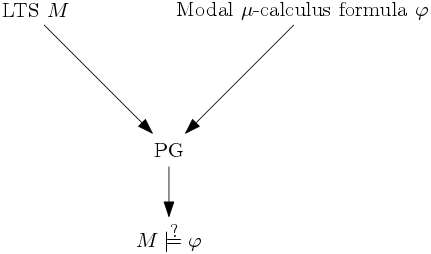
\includegraphics[scale=0.5]{Diagrams/LTSVerificationUsingPG}
	\caption[LTS verification using PG]{LTS verification using PG}
	\label{fig:ltsverificationusingpg}
\end{figure}


\subsection{Parity games}
\begin{definition}
	\label{def_PG}\cite{Bradfield2018}
	A parity game (PG) is a tuple $(V, V_0, V_1, E, \rho)$, where:
	\begin{itemize}
		\item $V = V_0 \cup V_1$ and $V_0 \cap V_1 = \emptyset$,
		\item $V_0$ is the set of vertices owned by player $0$,
		\item $V_1$ is the set of vertices owned by player $1$, 
		\item $E \subseteq V \times V$ is the edge relation,
		\item $\rho :  V \rightarrow \mathbb{N}$ is a priority assignment.
	\end{itemize}
\end{definition}
We write $\alpha \in \{0,1\}$ to denote an arbitrary player. We write $\overline{\alpha}$ to denote $\alpha$'s opponent, ie. $\overline{0} = 1$ and $\overline{1} = 0$.

A parity game is played by players 0 and 1. A play starts with placing a token on vertex $v \in V$. Player $\alpha$ moves the token if the token is on a vertex owned by $\alpha$, ie. $v \in V_\alpha$. The token can be moved to $w \in V$, with $(v,w) \in E$. A series of moves results in a sequence of vertices, called path. For path $\pi$ we write $\pi_i$ to denote the $i^{\text{th}}$ vertex in path $\pi$. A play ends when the token is on vertex $v \in V_\alpha$ and $\alpha$ can't move the token anywhere, in this case player $\overline{\alpha}$ wins the play. If the play results in an infinite path $\pi$ then we determine the highest priority that occurs infinitely often in this path, formally
\[ \max\{ p \ |\ \forall_j \exists_i j < i \wedge p = \rho(\pi_i) \}\] 
If the highest priority is odd then player $1$ wins, if it is even player $0$ wins.
\begin{figure}[h]
	\centering
	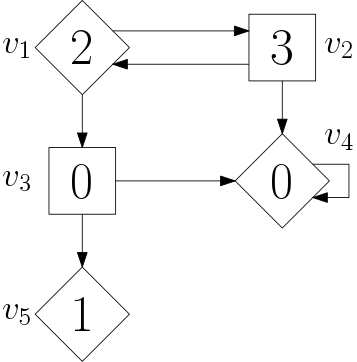
\includegraphics[scale=0.3]{Examples/SimplePG/PG}
	\caption[Parity game example]{Parity game example}
	\label{fig:simplepgpg}
\end{figure}

Figure \ref{fig:simplepgpg} shows an example of a parity game. We usually depict the vertices owned by player $0$ by diamonds and vertices owned by player $1$ by boxes, the priority is depicted inside the vertices. If the game starts by placing a token on $v_1$ we can consider the following exemplary paths:
\begin{itemize}
	\item $\pi = v_1v_3v_5$ is won by player $1$ since player $0$ can't move at $v_5$.
	\item $\pi = (v_1v_2)^\omega$ is won by player $1$ since the highest priority occurring infinitely often is 3.
	\item $\pi = v_1v_3(v_4)^\omega$ is won by player $0$ since the highest priority occurring infinitely often is $0$.
\end{itemize}


A strategy for player $\alpha$ is a function $\sigma : V^*V_\alpha \rightarrow V$ that maps a path ending in a vertex owned by player $\alpha$ to the next vertex. Parity games are positionally determined \cite{Bradfield2018}, therefore a strategy $\sigma: V_\alpha \rightarrow V$ that maps the current vertex to the next vertex is sufficient. 

A strategy $\sigma$ for player $\alpha$ is winning from vertex $v$ if and only if any play that results from following $\sigma$ results in a win for player $\alpha$. The graph can be divided in two partitions $W_0 \subseteq V$ and $W_1 \subseteq V$, called winning sets. If and only if $v \in W_\alpha$ then player $\alpha$ has a winnings strategy from $v$. Every vertex in the graph is either in $W_0$ or $W_1$ \cite{Bradfield2018}. Furthermore finite parity games are decidable \cite{Bradfield2018}.


\subsection{Creating parity games}
A parity game can be created from a combination of an LTS and a modal $\mu$-calculus formula. To do this we first examine some of the properties of the modal $\mu$-calculus. 

First we introduce the notion of unfolding, a fixpoint formula $\mu X . \varphi$ can be unfolded resulting in formula $\varphi$ where every occurrence of $X$ is replaced by $\mu X . \varphi$, denoted by $\varphi [ X:= \mu X . \varphi]$. A fixpoint formula is equivalent to its unfolding (\cite{Bradfield2018}), ie. for some LTS $[\![\mu X . \varphi]\!]^\eta = [\![\varphi[X:=\mu X . \varphi]]\!]^\eta$. The same holds for the fixpoint operator $\nu$.

Next we define alternating depth, this definition is literally taken from \cite{Bradfield2018}:
\begin{definition}
	The dependency order on bound variables of $\varphi$	is the smallest partial order such that $X \leq_\varphi Y$ if $X$ occurs free in $\sigma Y. \psi$ . The alternation depth of a $\mu$-variable X in formula $\varphi $ is the maximal length of a chain $X_1 \leq_\varphi  \dots \leq_\varphi X_n$ where $X = X_1$, variables $X_1, X_3, \dots$ are $\mu$-variables and variables $X_2, X_4, \dots$ are $\nu$-variables. The alternation depth of a $\nu$-variable is defined similarly. The alternation depth of formula $\varphi$, denoted $adepth(\varphi)$, is the maximum of the alternation depths of the variables bound in $\varphi$, or zero if there are no fixpoints.
\end{definition}
The example formula $\varphi = \nu X. \mu Y. ([ins]Y \wedge [std] X)$ which states that for an LTS with $Act = \{ ins, std\}$ the action std must occur infinitely often over all runs. Since $X$ occurs free in $\mu Y. ([ins] Y \wedge [std]X)$ we have $adepth(Y) = 1$ and $adepth(X) = 2$. As shown in \cite{Bradfield2018} we have find that formula $\mu X. \psi$ has the same alternation depth as its unfolding $\psi[X:=\mu X. \psi]$. Similarly for the greatest fixpoint.

We can now define the transformation from an LTS and a formula to a parity game. This relation is shown in the following diagram:

\begin{tikzpicture}
\matrix (m) [matrix of math nodes,row sep=4em,column sep=4em,minimum width=2em]
{
	\text{LTS} & \text{PG} \\};
\path[-stealth]
(m-1-1)
edge node [above] {$\varphi$} (m-1-2)
;
\end{tikzpicture}\\
\begin{definition}
	\label{def_LTS2PG}\cite{Bradfield2018}
	LTS2PG($M, \varphi$) converts LTS $M = (S, Act, trans, s_0)$ and closed formula $\varphi$ to a PG $(V, V_0, V_1, E, \rho)$.
	
	A vertex in the parity game is represented by a pair $(s, \psi)$ where $s \in S$ and $\psi$ is a modal $\mu$-calculus formula. We will create a vertex for every state with every subformula of $\varphi$ plus the unfoldings of fixpoint operators. Formally we define the set of vertices by first defining the set of subformula's:
	\[ F = \{ \psi\ |\ \psi \text{ is a subformula of } \varphi \} \text{, note that $\varphi$ is a subformula of $\varphi$,} \]
	and the set of unfolded fixpoint subformula's:
	\[ F_\sigma = \{\psi[X:=\sigma X. \psi]\ |\ \sigma X. \psi \in F \text{ with } \sigma \in \{\mu, \nu\}\} \]
	Having these sets we can define the set of vertices by:
	\[ V = S \times (F \cup F_{\sigma})\]
	
	We create the parity game with the smallest set $E$ such that:
	\begin{itemize}
		\item $V = V_0 \cup V_1$,
		\item $V_0 \cap V_1 = \emptyset$ and
		\item for every $v = (s, \psi) \in V$ we have:
		\begin{itemize}
			\item If $\psi = \top$ then $v \in V_1$.
			\item If $\psi = \bot$ then $v \in V_0$.
			\item If $\psi = \psi_1 \vee \psi_2$ then:
			\subitem $v \in V_0$,
			\subitem $(v, (s,\psi_1)) \in E$ and
			\subitem $(v, (s,\psi_2)) \in E$.
			\item If $\psi = \psi_1 \wedge \psi_2$ then:
			\subitem $v \in V_1$,
			\subitem $(v, (s,\psi_1)) \in E$ and
			\subitem $(v, (s,\psi_2)) \in E$.
			\item If $\psi = \langle a \rangle \psi'$ then $v \in V_0$ and for every $s \xrightarrow{ a} s'$ we have $(v, (s', \psi')) \in E$.
			\item If $\psi = [ a ] \psi'$ then $v \in V_1$ and for every $s \xrightarrow{ a} s'$ we have  $(v, (s', \psi')) \in E$.
			\item If $\psi = \mu X. \psi'$ then $(v, (s, \psi')) \in E$.
			\item If $\psi = \nu X. \psi'$ then $(v, (s, \psi')) \in E$.
			\item If $\psi = X$ then $(v, \sigma X. \psi') \in E$ where $\sigma X. \psi' \in F$.
		\end{itemize}
		Note that directing formula $\sigma X. \psi'$ to $\psi'$ and directing $X$ to $\sigma X. \psi'$ is equivalent to using unfolding which would direct $\sigma X. \psi'$ to $\psi'[X:=\sigma X. \psi']$.
	\end{itemize}
	
	
	Finally we have $\rho(s, \psi) = \begin{cases}
	2 \lfloor adepth(X) / 2 \rfloor & \text{if } \psi = \nu X. \psi'\\
	2 \lfloor adepth(X) / 2 \rfloor + 1 & \text{if } \psi = \mu X. \psi'\\
	0 & \text{otherwise}
	\end{cases}$
\end{definition}
\begin{figure}[h]
	\centering
	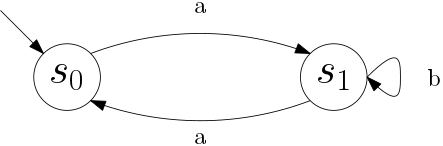
\includegraphics[scale=0.3]{Examples/ExamleVerification/LTSprojempty}
	\caption[LTS $M$]{LTS $M$}
	\label{fig:exverltsprojempty}
\end{figure}
Consider the LTS in figure \ref{fig:exverltsprojempty} and formula $\varphi = \mu X.[a]X \vee \langle b \rangle \top$ expressing that on any path reached by a's can eventually do a b action. We will use this as a working example in the next few sections. The resulting parity game is depicted in figure \ref{fig:exverpg}. Solving this parity game results in the following winning sets:
\begin{align*}
W_0 = \{& (s_1, \mu X.[a]X \vee \langle b \rangle \top)\\
& (s_1, [a]X \vee \langle b \rangle \top)\\
& (s_1, [a]X)\\
& (s_1, X)\\
& (s_1, \top)\\
& (s_2, \mu X.[a]X \vee \langle b \rangle \top)\\
& (s_2, [a]X \vee \langle b \rangle \top)\\
& (s_2, [a]X)\\
& (s_2, X)\\
& (s_2, \langle b \rangle \top)\\
& (s_2, \top)\\
 \}\\
W_1 = \{& (s_1, \langle b \rangle \top )\}
\end{align*}
With the strategies $\sigma_0$ for player $0$ and $\sigma_1$ for player $1$ being (vertices with one outgoing edge are omitted):
\begin{align*}
\sigma_0 = \{
&(s_1, [a]X \vee \langle b \rangle \top) \mapsto (s_1, [a] X), \\
&(s_2, [a]X \vee \langle b \rangle \top) \mapsto (s_2, \langle b \rangle \top) \} \\
\sigma_1 = \{\} \\
\end{align*}
\begin{figure}[h]
	\centering
	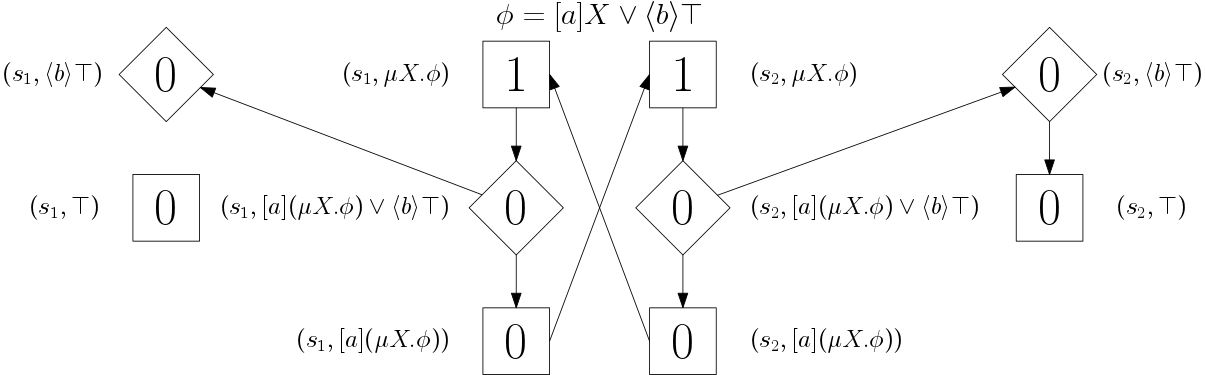
\includegraphics[scale=0.3]{Examples/ExamleVerification/PG}
	\caption[Parity game resulting from $M$ and $\varphi$]{Parity game resulting from $M$ and $\varphi$}
	\label{fig:exverpg}
\end{figure}

State $s$ in LTS $M$ only satisfies $\varphi$ iff player $0$ has a winning strategy from vertex $(s, \varphi)$. This is formally stated in the following theorem which is proven in \cite{Bradfield2018}.
\begin{theorem}
	\label{the_LTS_PG_REL}Given LTS $M = (S, Act, trans, s_0)$, modal $\mu$-calculus formula $\varphi$ and state $s \in S$ it holds that $M, s \models \varphi$ iff $s \in W_0$ for the game $LTS2PG(M, \varphi)$.
\end{theorem}

\subsection{FTSs and parity games}
Using the theory we have seen thus far we can verify FTSs. Namely by verifying every projection of the FTS to a valid product. This relation is depicted in the following diagram where $\Pi$ indicates a projection:
\\\begin{tikzpicture}
\matrix (m) [matrix of math nodes,row sep=4em,column sep=4em,minimum width=2em]
{
	\text{FTS} \\
	\text{LTS} & \text{PG} \\};
\path[-stealth]
(m-1-1) edge [double] node [left] {$\Pi$} (m-2-1)
(m-2-1.east|-m-2-2) edge node [above] {$\varphi$}
(m-2-2)
;
\end{tikzpicture}\\
As mentioned before verifying products dependently is potentially more efficient. In the next two sections we define an extension to parity games, namely \textit{variability parity games} (VPG) which can be used to verify an FTS. We will translate an FTS and a formula into a VPG which solution will provide the information needed to conclude for which products the FTS satisfies the formula. This relation is depicted in figure \ref{fig:ftsverificationusingvpg}.
\begin{figure}[h]
	\centering
	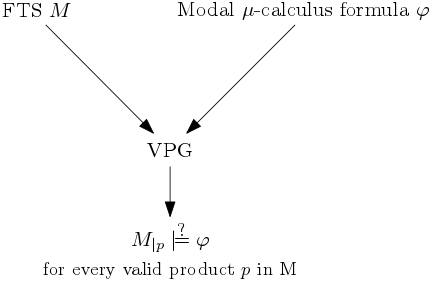
\includegraphics[scale=0.5]{Diagrams/FTSVerificationUsingVPG}
	\caption[FTS verification using VPG]{FTS verification using VPG}
	\label{fig:ftsverificationusingvpg}
\end{figure}
